\section{Introduction}
\label{sec:intro}


The Gauss-Bonnet theorem states that the sum of the curvature
at each point on a surface is $2\pi$ times the Euler characteristic.
The theorem is a bridge between topological
and geometric information, see \figref{bridge}. 
This bridge can be traversed in both directions.
That is, if one has geometric information one can deduce topological information and
if one has topological information one can deduce geometric information.


\begin{figure}[htb]
\centering
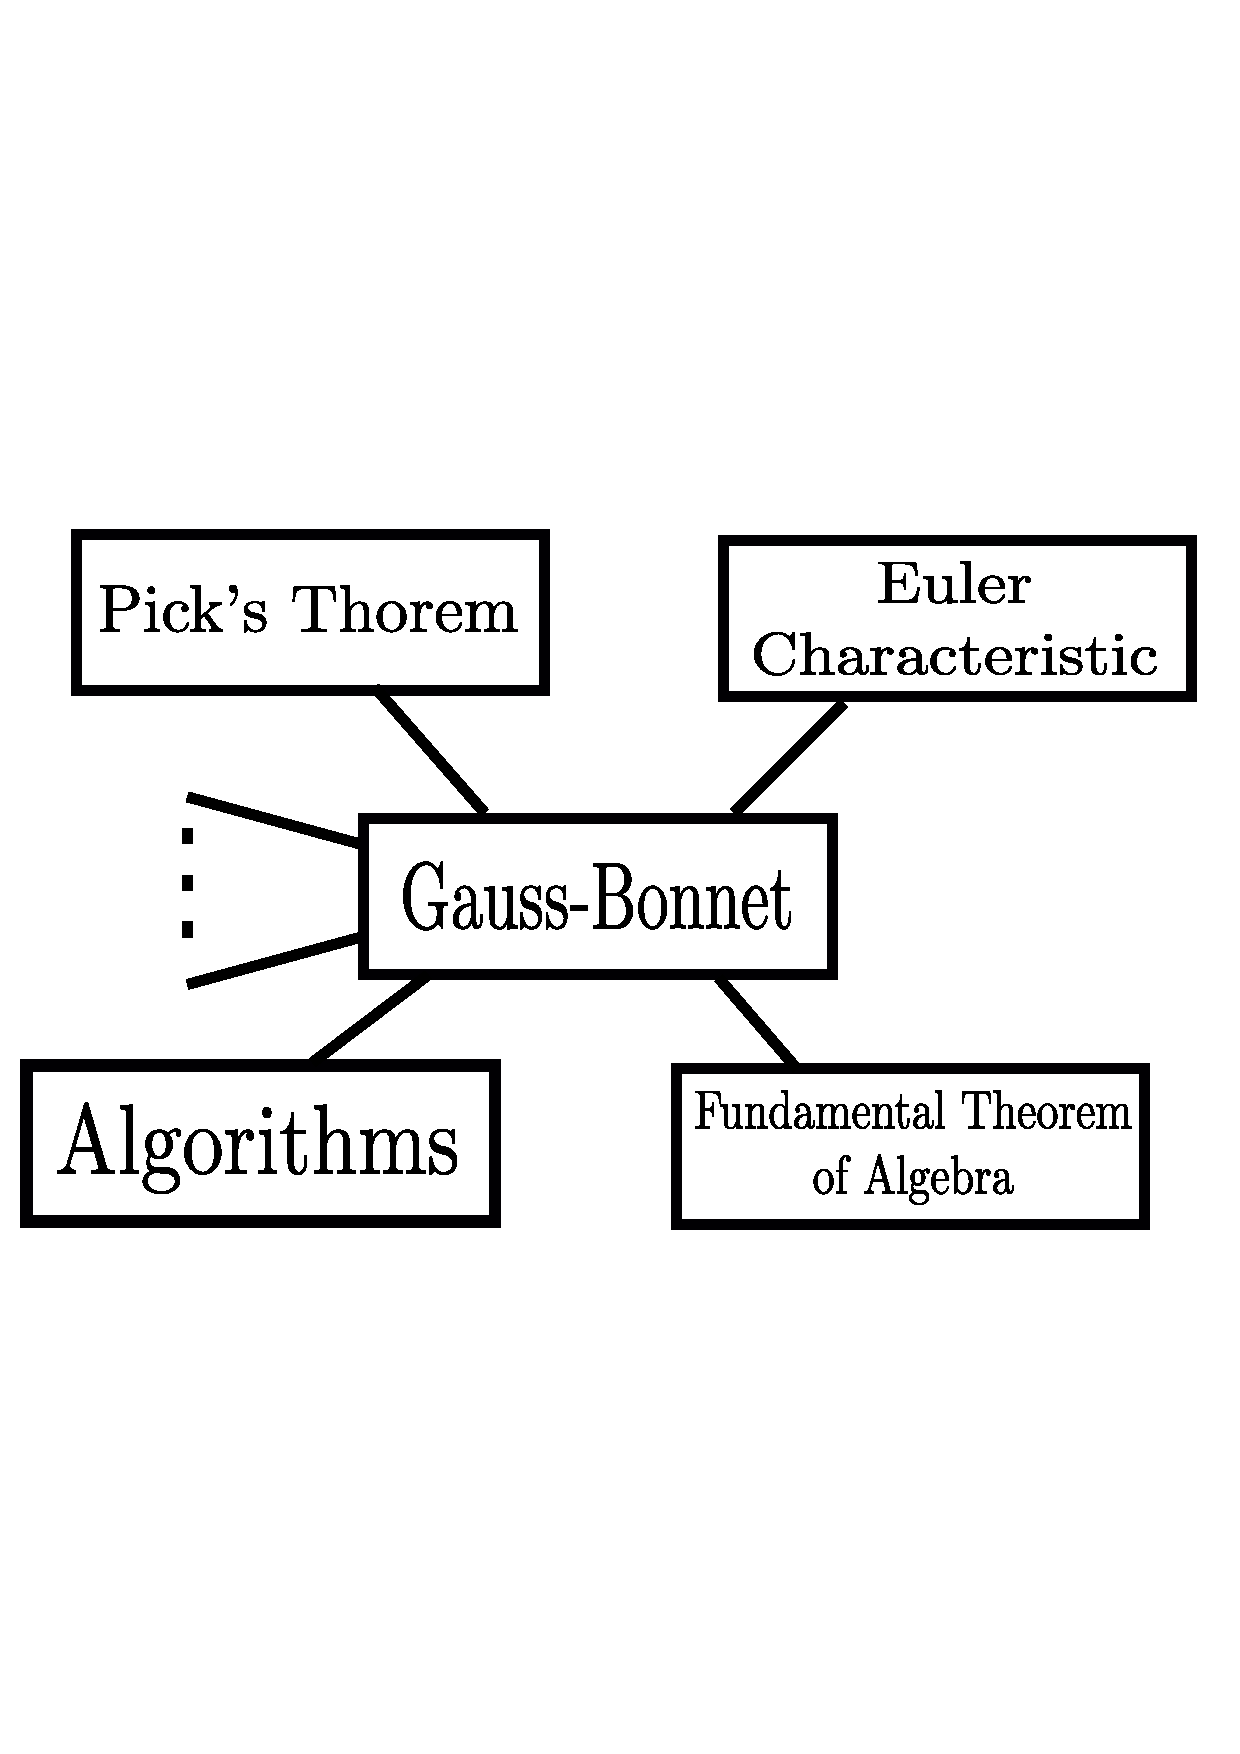
\includegraphics[width=.3\textwidth]{curvature/bridge}
\caption{The Gauss-Bonnet theorem allowing bi-directional traffic
between geometry and topology.}
\label{fig:bridge}
\end{figure}

This work is inspired by Matou\v{s}ek's book \emph{Using the Borsuk-Ulam Theorem}
\cite{jm08}.
Matou\v{s}ek states that a theorem is a great theorem if there are
\begin{enumerate}[(1)]
\item several different equivalent versions,
\item many different proofs,
\item a host of extensions and generalizations, and
\item numerous interesting applications.
\end{enumerate}

By this criteria, the Gauss-Bonnet theorem is a great theorem.
For (1), six\todo{verify} different versions of the theorem are discussed
in \cite{wu_historical_2008}. 
We highlight a discrete version version of the theorem that leads to several
results in algorithms.

As for (2), the most common proof is to first prove the theorem for simply connected domains
with boundary, then triangulate a surface and add up the contribution from each triangle.
We will give an elementary proof of a version of the theorem using this strategy.
Several fundamentally different proofs exist, for example 
a proof based on the calculus of
moving surfaces is given in \cite{grinfeld_introduction_2013}.
For (3), several generalizations exist. Two examples include
the Chern-Gauss-Bonnet theorem \cite{chern_simple_1944} and the celebrated Atiyah–Singer index 
theorem \cite{atiyah_index_1963}.
This work is dedicated to (4).

This paper is organized as follows:
in \secref{background} we introduce definitions and notation that will be used
throughout the paper. We then state and prove the theorem.
In each subsection of \secref{applications}, we present an application of the theorem.
In general, the sections containing applications are ordered from simpler to more technical,
and are independent.


I hope that the number of applications continues to grow,
please share any that you feel
ought to be included\footnote{\text{bradleymccoy@montana.edu}}.
Most of our applications are related to algorithms. 
Several applications of the continuous version of the theorem
are given in \cite{doc76,pressley_elementary_2010}, for applications of the Gauss-Bonnet 
theorem in physics see \cite{tirado-physics-apps,gibbons_applications_2008}.
For a historical survey of the theorem from Gauss to Chern see  \cite{wu_historical_2008}.